\documentclass[conference]{IEEEtran}
% SC-length version (10 pages + references) of main_v2.tex (full length); details are in supplement.tex.
% Build: paper/build.sh main_sc
% Figures: gh200/analysis/paper_figures.py and mi350/analysis/paper_figures_mi350.py -> figs/
\usepackage{cite}
\usepackage{amsmath}
% Times-compatible fonts under XeTeX (IEEEtran's ptm Times is not available in the TU encoding tectonic uses)
\usepackage{fontspec}
\setmainfont{texgyretermes}[Extension=.otf,UprightFont=*-regular,BoldFont=*-bold,ItalicFont=*-italic,BoldItalicFont=*-bolditalic]
\setsansfont{texgyreheros}[Extension=.otf,UprightFont=*-regular,BoldFont=*-bold,ItalicFont=*-italic,BoldItalicFont=*-bolditalic]
\setmonofont{texgyrecursor}[Extension=.otf,UprightFont=*-regular,BoldFont=*-bold,ItalicFont=*-italic,BoldItalicFont=*-bolditalic]
\usepackage{unicode-math}
\setmathfont{texgyretermes-math.otf}
\usepackage{graphicx}
\usepackage{booktabs}
\usepackage{multirow}
\usepackage{url}
\usepackage{xcolor}
\usepackage[hidelinks]{hyperref}

\newcommand{\W}{\,W}
\newcommand{\Eh}{\,E$_\mathrm{h}$}
\newcommand{\Ry}{\,Ry}
\newcommand{\ee}[2]{#1{\times}10^{#2}}  % \ee{1.2}{-5} -> 1.2x10^-5 (math mode)
\newcommand{\pct}{\%}
% Results of experiments still running when this draft was written; every occurrence must be gone before submission.
\newcommand{\pending}[1]{\textcolor{red}{[pending: #1]}}

\begin{document}
\bstctlcite{IEEEexample:BSTcontrol}

\title{Unused Mantissa Bits on Power-Capped GPUs: Mechanism, Prediction and Limits on NVIDIA GH200 and AMD MI350X}

\author{\IEEEauthorblockN{Koying Chen}
\IEEEauthorblockA{Department of Computer Science, National Tsing Hua University, Hsinchu, Taiwan}}
% Double-blind submission: replace the author block with "Anonymous" before submitting.

\maketitle

\begin{abstract}
When a GPU runs at its power limit, the energy of every operation sets the clock. We study a format-preserving way to
lower that energy: zeroing, in software, the low-order mantissa bits an application does not need, on the original
FP64, BF16 or FP8 units. On an NVIDIA GH200 cluster and two 8-GPU AMD MI350X nodes, filling the discarded bits with ones
instead of zeros, which stops them toggling without making them zero, retains 65--97\pct{} of the saving: switching
activity is the main contributor. A two-parameter model built on this predicts a truncated kernel's speedup under every
cap from the native curve, the idle power and one or two measurements, within 1.5 and 2.1 percentage points on average
on GEMMs and 1.6 on two applications not used to develop it.
MI350X is power-bound at its stock 1000\W{} limit, so truncation pays at default settings: 4.6--5.1\pct{} for FP64 HPL (36
significand bits), 4.9--5.1\pct{} for HPL-MxP on a diagonally dominant test matrix (3 BF16 bits), 7.4\pct{} for a
Gaussian-process likelihood and 10\pct{} for DF-MP2, and 7--19\pct{} at 500\W, with every accuracy check passed. It is not
always the best choice. INT8 emulation of FP64 (GEMMul8) makes HPL 36\pct{} and DF-MP2 67\pct{} faster than native at
1000\W, but it is slower than native when the inner dimension is 1024 (the Gaussian process: $-11\pct$), loses most of its
lead under a tight cap (HPL at 500\W: 4\pct{} ahead of truncation), needs workspace that limits problem size, and can fail
silently, through precision loss on wide per-row exponent spans or, in the build we used, a size overflow. Which method wins is set by shape, cap, memory and precision; truncation is the one that keeps the format and
also applies to BF16 and FP8, for which no emulation exists.
\end{abstract}

\begin{IEEEkeywords}
power capping, energy efficiency, floating-point precision, mantissa truncation, GPU, mixed precision, HPL, emulation
\end{IEEEkeywords}

%==================================================================================================
\section{Introduction}

Power is becoming the ceiling on delivered performance. Data centers cap rack power, competitions cap cluster power,
and accelerators ship with package limits that their own workloads reach: the AMD Instinct MI350X holds FP64, BF16 and
FP8 matrix multiplication at its default 1000\W{} limit 82--100\pct{} of the time in our measurements. Under a limit the
power manager lowers the clock until the device fits, so the speed of a program depends on how much energy each of its
operations consumes.

That GPU power depends on input data is known: DGEMM on random operands draws 67\pct{} more power than on constant
ones on A100~\cite{Bhalachandra2022}; zeroing the least significant bits of GEMM inputs lowers power~\cite{Gregersen2024};
an all-zero GEMM runs about 15\pct{} faster than a random one on A100, more so at lower power limits~\cite{He2024}; and
a zero-input DGEMM on GH200 draws 563 instead of 898\W~\cite{Antepara2025}. Hardware designs narrow multipliers or mask
mantissas at unit inputs~\cite{Tong2000,Pool2011,Guenther2016,AMD2022}. These works use all-zero or constant data on one
vendor, or need new hardware. They leave open what a practitioner needs to know: whether software truncation of
\emph{real} data buys performance on production GPUs of different vendors, and through which mechanism; whether the gain
can be predicted without measuring every variant under every cap; what it costs in accuracy; and where it still pays off
against format changes such as INT8 emulation of FP64~\cite{Ozaki2025,Uchino2025}, whose speed also depends on the power
limit. Our contributions are:

\begin{enumerate}
\item \textbf{Evidence on the mechanism across vendors, units and clocks.} Fills that stop the discarded bits toggling
without making them zero retain 65--97\pct{} (ones) and 41--92\pct{} (fixed pattern) of the saving in matrix engines, FP64
vector units and memory copies on GH200 and MI350X (Section~\ref{sec:why}); on MI350X truncation also raises the effective
clock at a fixed target clock, a reduction no throttle counter reports.
\item \textbf{A predictive model.} If truncation only changes the switched capacitance, the truncated program under cap
$P$ behaves like the native program under $P_0+(P-P_0)/R$. With $P_0$ the measured idle power, it predicts 42
cap--format points per platform with mean errors of 1.5 and 2.1 percentage points (Section~\ref{sec:model}).
\item \textbf{Deployable gains on real applications on two platforms.} In-program truncation, measured against the
unmodified program with paired designs, replicated on a second node set or node, speeds up HPL, HPL-MxP, Quantum ESPRESSO,
DF-MP2 and a Gaussian-process likelihood, with each code's own accuracy criterion met (Section~\ref{sec:results}). On
MI350X the gains appear at the default limit.
\item \textbf{A head-to-head comparison with INT8 emulation.} At the best configuration each method allows, emulation
wins for long inner dimensions at generous caps (HPL at 1000\W: 576.8 against 444.6\,TFLOP/s for truncation); a tighter
cap, small inner dimensions, limited memory, many distinct shapes and wide per-row exponent spans favor truncation, and
for BF16 and FP8 it is the only option (Section~\ref{sec:format}, Table~\ref{tab:h2h}).
\item \textbf{Measurement lessons.} Hardware energy accumulators avoid sampling bias; chassis fans that react to the
previous run change a power-capped GPU's speed by up to 4.5\pct{} through its temperature, which interleaving alone does
not remove; and safe bit counts must be validated per platform (Sections~\ref{sec:setup}, \ref{sec:hpl}).
\end{enumerate}

%==================================================================================================
\section{Background and Related Work}\label{sec:related}

\textbf{Input-dependent power.} Gregersen et al.\ varied value distribution, bit similarity and sparsity of GEMM inputs
on A100, H100 and V100 and saw power differ by almost 40\pct, but avoided throttling~\cite{Gregersen2024}; He swept the
A100 power limit~\cite{He2024} and Antepara et al.\ measured GH200~\cite{Antepara2025,Antepara2025W}, both with all-zero
versus random inputs; Lucas and Juurlink modeled ALU power by the number of toggles~\cite{Lucas2016}. None truncates real
data, evaluates accuracy or applications, or compares vendors.

\textbf{Power-constrained HPC.} Manufacturing variation makes processors differ under the same power
bound~\cite{Rountree2012,Inadomi2015}; overprovisioning~\cite{Patki2013} and power-limit tuning~\cite{Zeus2023} decide
how power is distributed. We lower the energy each operation needs, so the two compose.

\textbf{Masking, precision tuning and data movement.} Mantissa masking in hardware saves energy in
multipliers~\cite{Tong2000}, shaders~\cite{Pool2008,Pool2011,Angerd2017}, baseband processors~\cite{Guenther2016} and
register files~\cite{Jahadi2024}; DRAM and HBM energy depend on toggling~\cite{Chatterjee2017,OConnor2017,Ghose2018}. Precision
tuning~\cite{RubioGonzalez2013}, mixed-precision storage~\cite{Higham2022,Grutzmacher2020} and transprecision
computing~\cite{Malossi2018} change types or bytes; zeroing changes neither. Low-precision LU with refinement underlies
HPL-MxP~\cite{Haidar2018,Dongarra2025}, and bit-information analysis can estimate needed bits from data~\cite{Klower2021}.

\textbf{FP64 emulation and format changes.} The Ozaki scheme splits a product into exactly computed low-precision
slices~\cite{Ozaki2012,Ootomo2024}; Ozaki scheme~II uses modular arithmetic~\cite{Ozaki2025} and is implemented in
GEMMul8 for CUDA and HIP~\cite{Uchino2025}; cuBLAS ships a fixed-point emulation with an automatic mode that picks the
bit count from the exponent span~\cite{cuBLASEmu,Schwarz2026}. Tile mixed precision converts whole tiles of geostatistics
factorizations to lower formats~\cite{Abdulah2019,Abdulah2022,Cao2022,Cao2023,Ren2025}, and convergence-driven schemes
switch formats or slice counts by solver state~\cite{Woo2023,Huang2026}. All of these change the format; truncation keeps
the original units, so the two can compose.

%==================================================================================================
\section{Why Fewer Mantissa Bits Save Power}\label{sec:why}

Dynamic power is roughly $\alpha_\mathrm{sw} C V^2 f$ with a data-dependent switching activity $\alpha_\mathrm{sw}$.
Under a cap the power manager lowers $f$ (and $V$) until the device fits, so a lower $\alpha_\mathrm{sw}$ becomes clock;
below the cap it appears as lower power. Both occur on both platforms. On GH200 at its default 1000\W{} module cap the
native FP64 GEMM is capped 95\pct{} of the time at 1822\,MHz; with 0 kept bits it runs at the maximum 1980\,MHz while
module power falls from 984 to 707\W. On MI350X at its default 1000\W{} package limit the native FP64 GEMM is held at the
limit 82\pct{} of the time at 1890\,MHz; with 0 kept bits it draws 785\W{} at 2183\,MHz and is 17\pct{} faster.

\textbf{Toggling or zero?} Zeroing stops the low bits from varying and makes them zero. Filling them with ones or a
fixed nonzero pattern instead also stops them toggling but is not zero. On GH200 we compare module power at 1000\W{} or
throughput at 500\W; on MI350X we lock the maximum graphics clock at 900, 1300 or 1700\,MHz, below the frequency any
configuration reaches, so that none is power-limited (PPT residency 0--0.6\pct) and the energy per operation compares
switching activity directly (8 GPUs $\times$ ABBA).

\begin{table}[t]
\caption{Share of the zero-fill benefit (\%) retained by a fill with ones / a fixed pattern. GH200: module power at
1000\W{} or throughput at 500\W; MI350X: energy per operation at locked clocks (GEMMs, range over three clocks),
throughput at 600\W{} or power at 1000\W{} (other kernels). Last column: zero-fill benefit on MI350X (E/op: energy per
operation).}\label{tab:fill2}
\centering\footnotesize\setlength{\tabcolsep}{3pt}
\begin{tabular}{@{}lccr@{}}
\toprule
Kernel, kept bits & GH200 & MI350X & MI350X zero fill \\
\midrule
FP64 GEMM, 0 & 76/68 & 73--75/69 & $-20$ to $-29\pct$ E/op \\
FP64 GEMM, 20 (G), 27 (M) & 87/82 & 81--83/73--74 & $-7$ to $-10\pct$ E/op \\
BF16 GEMM, 0 & 92/92 & 77--78/68--72 & $-13$ to $-15\pct$ E/op \\
FP8 GEMM, 0 & --- & 65--66/61 & $-9$ to $-10\pct$ E/op \\
FP64 FMA loop, 0 & 87/62 & 74/63 & +33\pct{} speed \\
Memory copy, 0 & 97/86 & 83/41 & $-9\pct$ power \\
\bottomrule
\end{tabular}
\end{table}

Most of the benefit survives such fills, in matrix engines, FP64 vector units and memory copies of both vendors
(Table~\ref{tab:fill2}): switching activity, not the value zero, is the main contributor, quantitative support for the
toggling hypothesis~\cite{Gregersen2024} beyond one vendor or unit. The shares are not an exact causal decomposition: a
fill also changes partial products, alignment and accumulation inside the units, and shares measured as power and as
capped throughput need not add up. On MI350X the shares barely change with the clock (FP64, 27 bits: 83, 81 and 82\pct{}
at 900, 1300 and 1700\,MHz), while the total saving grows with it (FP64, 0 bits: 20, 24 and 29\pct{} less energy per
operation), as expected when $CV^2f$ grows relative to static power. Zeros save somewhat more than ones, consistent with
partial products $a_ib_j$ in which fixed ones still toggle against the other operand's kept bits; we have no gate-level
measurement. The effect is not limited to matrix engines: an FP64 multiply-add loop with 0 kept bits draws 553 instead
of 862\W{} on GH200 at 1000\W{} and runs 33\pct{} faster on MI350X at 600\W, and a memory copy, power-bound on MI350X at
600\W, runs 28\pct{} faster.

\textbf{A second clock effect on MI350X.} With the clock locked and nothing power-limited, the effective clock still
depends on the data: at a 1300\,MHz lock the native FP64 GEMM runs steadily at 1171--1179\,MHz (5th--95th percentile, 8
GPUs) and with 0 kept bits at 1235--1240\,MHz; native BF16 at 1088--1100 and with 0 bits at 1132--1142\,MHz, at
59--63\,\textdegree C. Power and thermal residency read zero, and the per-XCD ``clock below host limit'' counters stay
zero even while the power limit is active, so no available counter reports this reduction. Circuit-level clock
stretching under supply droop would explain it; we have no direct measurement. Truncation relieves it too.

%==================================================================================================
\section{A Model of Truncation Gains Under a Power Cap}\label{sec:model}

Let a GPU under cap $P$ settle at a target clock $f$. Its voltage $V(f)$ is set by the target clock, but switching
happens at the effective clock $sf$, where $s\le1$ is the data-dependent clock reduction of Section~\ref{sec:why}
($s=1$ when there is none). With $c$ the program's effective switched capacitance and $P_0$ the power that does not scale
with switching,
\begin{equation}
P = P_0 + c\,s\,V(f)^2 f = P_0 + c\,s\,g(f),
\end{equation}
and performance is proportional to $sf$. Truncation changes $c$ and $s$, not $g$. For the native ($n$) and truncated ($r$)
program define
\begin{equation}
R=\frac{c_rs_r}{c_ns_n},\qquad \sigma=\frac{s_r}{s_n};
\end{equation}
at a common locked target clock, $R$ is the ratio of their dynamic powers and $\sigma$ the ratio of their effective
clocks, both directly measurable. Under cap $P$ the truncated program settles where $c_rs_rg(f_r)=P-P_0$; the native
program reaches the same target clock $f_r$ under $P'$ with $c_ns_ng(f_r)=P'-P_0$. Dividing,
\begin{gather}
P'=P_0+\frac{P-P_0}{R},\qquad p_r(P)=\sigma\,p_n(P'),\\
\Delta W=P'-P=(P-P_0)\left(\tfrac{1}{R}-1\right),
\end{gather}
where $p_r(P)=\sigma\,p_n(P')$ because both run at target clock $f_r$ and performance scales with $s$. The model assumes
that $s$ does not change with $f$ over the range used and that the program stays compute-bound; predictions are capped
at the program's clock-limited peak. The model needs the native curve $p_n(P)$ and $P_0$; it saves measuring every
truncated variant under every cap. We set $P_0$ to the measured idle power, independent of the validation data: 174\W{}
for a GH200 module (three nodes 169--179\W) and 262\W{} per MI350X GPU. The truncated kernel is characterized by
locked-clock runs at 1300\,MHz (MI350X; $R$, $\sigma$; no point of the cap sweep) or by its speed at the lowest cap
(GH200, which we could not clock-lock; $\sigma=1$; that point is excluded from evaluation), and predictions are compared
with the GEMM sweeps at the other caps.

\begin{figure}[t]
\centering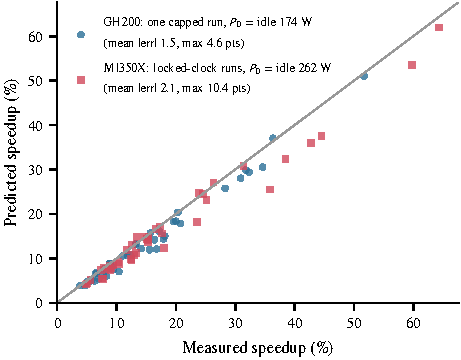
\includegraphics[width=\columnwidth]{figs/mi350_model.pdf}
\caption{Predicted against measured GEMM speedups under caps (FP64 with 0, 12/27 and 35/36 kept bits, BF16 with 0 and
3, FP8 with 0), with $P_0$ set to the measured idle power.}\label{fig:model}
\end{figure}

\begin{table}[t]
\caption{Model error in percentage points of speedup over 42 cap--format points per platform. Idle: $P_0$ = measured
idle power; LOO: $P_0$ fitted on all other formats and applied to the held-out one; zero: all power treated as
dynamic. Last column: largest error for FP64 with 27--36 kept bits.}\label{tab:modelerr}
\centering\footnotesize\setlength{\tabcolsep}{4pt}
\begin{tabular}{@{}llrrrr@{}}
\toprule
Platform & $P_0$ & Mean & Max & Max, FP64 27--36 \\
\midrule
GH200 & idle 174\W & 1.5 & 4.6 & 2.9 \\
GH200 & LOO (190--200\W) & 1.0 & 3.6 & --- \\
GH200 & 0 & 6.1 & 12.9 & --- \\
MI350X & idle 262\W & 2.1 & 10.4 & 2.9 \\
MI350X & LOO (190--250\W) & 2.3 & 9.4 & --- \\
MI350X & 0 & 4.0 & 17.2 & --- \\
\bottomrule
\end{tabular}
\end{table}

The mean absolute error is 1.5 percentage points on GH200 (largest 4.6) and 2.1 on MI350X (largest 10.4;
Fig.~\ref{fig:model}, Table~\ref{tab:modelerr}). Fitting $P_0$ on all other formats and predicting the held-out one gives 1.0 and 2.3; treating all
power as dynamic ($P_0=0$) gives 6.1 and 4.0, and omitting $\sigma$ on MI350X 2.5. The ratios are $R=0.94$, 0.89 and 0.67
for FP64 with 36, 27 and 0 kept bits, 0.92 and 0.85 for BF16 with 3 and 0, 0.90 for FP8 with 0, and $\sigma=1.01$--1.05.
For the FP64 widths applications keep (27--36 bits) the error is at most 2.9 points on both platforms; it is largest for
BF16 with 0 bits at 400\W{} on MI350X, where the native GEMM barely runs, and for FP64 with 0 bits at 500--800\W, whose
clock exceeds anything on the native curve. \textbf{External validation.} The GEMM points were used to develop the model. As a test on programs that played no part
in it, we ran DF-MP2 and the Gaussian-process likelihood at the 1300\,MHz lock on node n02, derived $R$ and $\sigma$ from
their whole-program power and clock ($R=0.92$ and 0.86, $\sigma=1.01$ and 1.02 for DF-MP2 with 32 and 20 bits; $R=0.96$ and
0.93 for the likelihood with 36 and 28 bits), and predicted their speedups at 500--1000\W{} from their native curves on the
same node. Over the 16 points the mean error is 1.6 percentage points and the largest 3.6. DF-MP2 is predicted within
$-1.6$ to $+2.4$ points; the likelihood is underpredicted at every cap, by 0.6--3.6 points, perhaps because its Cholesky
alternates GEMM-heavy and non-GEMM phases whose power differs, which one whole-program ratio does not capture. Once a
platform's idle power and an application's native curve are known, a truncated program's curve thus follows from one
locked-clock run to within a few points, and $\Delta W\propto P-P_0$ explains why the equivalent saving grows with the cap
where the relative speedup does not.

%==================================================================================================
\section{Method and Experimental Setup}\label{sec:setup}

\textbf{Truncation.} We keep the top $k$ of the $p$ fraction bits of an operand (52 for FP64, 7 for BF16, 3 for FP8
E4M3) and zero the rest, by truncation (a bit mask) or round-to-nearest (add half a unit of the last kept bit first);
sign and exponent are untouched. HPL counts significand bits including the hidden bit (36 bits = 35 fraction bits) and
rounds to nearest even; applications round to nearest; GEMM microbenchmarks and HPL-MxP truncate. For uniform operands the
relative error of $C=AB$ is $\approx\alpha2^{-k}$ with $\alpha\approx0.27$ (nearest) or 0.70 (truncation), independent of
the inner dimension; truncation's error is a systematic shrinkage, which solvers with residual correction tolerate but
accumulating processes do not. On real data $\alpha$ ranges from 0.07 to 9.6 with cancellation, so tolerable bit counts
must be measured per application. The equivalent saving $\Delta W(P)=P_\mathrm{native}(p'(P))-P$ is the extra cap the
native program needs to match the truncated one, interpolated along the native curve. For plane-wave DFT we tie the bit
count to the Davidson threshold $\mathit{ethr}$: $k=\mathrm{clamp}(\lceil-\log_2\mathit{ethr}\rceil+m,16,52)$.

\textbf{GH200.} Fourteen nodes with one GH200 480GB superchip each (Hopper GPU, maximum SM clock 1980\,MHz, FP64 tensor
peak 67\,TFLOP/s~\cite{NVIDIAGH200}), 200\,Gb/s InfiniBand, NVHPC 26.5 (CUDA 13.2). The module cap (GPU, CPU and memory)
is set from 200 to 1000\W; the default is also the maximum.

\textbf{MI350X.} Two nodes with eight MI350X OAM GPUs each (gfx950, 288\,GB HBM3E, maximum clock 2200\,MHz), ROCm 7.2.3,
Open MPI 5.0.7 with UCX. The per-GPU package limit is set from 1 to 1000\W; the default is the maximum; idle power is
244--275\W{} per GPU.

\textbf{Workloads.} GEMM microbenchmarks with cuBLAS or rocBLAS/hipBLASLt on uniform operands (FP64
$32768^2{\times}2048$; BF16 and FP8 $32768^2{\times}k$ with $k=6144$ or 8192). HPL and HPL-MxP: on GH200 8 nodes (HPL tuned,
$N=286720$; HPL-MxP $N=491520$); on MI350X one node of 8 GPUs (HPL $N=540672$, $1\times8$; HPL-MxP $N=1034752$,
7.6\,PFLOP/s natively); HPL-MxP uses a diagonally dominant test matrix, which its rules allow for testing
only~\cite{HPLMxPRules}. Quantum ESPRESSO 7.6~\cite{Giannozzi2020} (Si\,1000 at 550\W, Au\,112 at 450\W; GH200).
DF-MP2 for taxol def2-TZVP (113 atoms): GPU4PySCF~\cite{Wu2025} on GH200; on MI350X, where GPU4PySCF does not run, the
same three-index tensor built by PySCF on the CPU and contracted on the GPU (energy within $\ee{2}{-13}$\Eh{} of PySCF and
$\ee{7.5}{-8}$\Eh{} of GPU4PySCF). An ExaGeoStat-like Gaussian-process likelihood on both ($n=80000$, Matérn-3/2,
blocked Cholesky with one FP64 DGEMM per panel). Truncation happens inside each program; GEMMul8~\cite{Uchino2025} and
cuBLAS emulation replace FP64 GEMMs through a hook or the math mode.

\textbf{Measurement.} GH200: nvidia-smi samples every 250--500\,ms, and energy integrates 1-s averaged module power.
MI350X: a sampler reads all eight GPUs every 100\,ms, including a 15.26-$\mu$J hardware energy counter (energy is its
difference across a window) and the residency of power and thermal limiting. Every run records the cap in effect.
Variants run in ABBA order on the same nodes or GPUs after a cool-down; on MI350X all 8 GPUs run the same configuration
at once.

\textbf{A pitfall: fans and temperature.} On MI350X at 800\W{} a three-variant ABBA sequence of HPL-MxP made 4 kept bits
look faster than 3. After a hot run the chassis fans speed up, the junction temperature falls by 25\,\textdegree C within
20\,s, the cool-down condition is met at once, and the next run stays about 12\,\textdegree C cooler; the middle variant
always followed a hot run. Pairwise ABBA blocks with a minimum rest reduced but did not remove the effect: the run after a
hot run was still up to 15\,\textdegree C cooler and up to 4.5\pct{} faster, because cooler silicon leaks less and leaves
more of the budget for switching. Temperature thus enters in two ways that must not be confused. Differences caused by
the previous run and the fans are a confounder; differences caused by the truncated program itself drawing less power
are part of its benefit, but only where it is not power-bound (under a binding cap both draw the cap). We report two
quantities. The \emph{gain in the same cooling environment} is the raw paired ratio, measured under the chassis' own fan
control; it is what a user obtains. The \emph{data effect at equal temperature} regresses log performance on the variant
and the run's mean junction temperature within each cap (coefficient $-0.1$ to $-0.9\pct$ per \textdegree C), which removes
the confounder but, where truncation itself cools the GPU, also part of the benefit. Equal mean temperature does not imply
equal fan speed or thermal history, so we also control the history directly: before every run, all variants execute the
same fixed thermal load (a 3-minute native BF16 GEMM on all 8 GPUs), and key GEMM comparisons run 4 minutes before a
2-minute window so that each settles at its own steady state. We could not fix the fan speed.

\textbf{Statistics.} Each speedup is a paired ratio on the same node, cap and ABBA round. Measurements that share a
chassis or a job are not independent, so on MI350X the unit is one measurement window of all 8 GPUs (GEMM), one node run
(HPL, HPL-MxP) or one round of all 8 GPUs (GP, DF-MP2), and every MI350X experiment is repeated on the second node. On
GH200 the units are node--pair samples from two node sets (HPL, HPL-MxP) or three nodes (GEMM), which treats pairs within
a job as independent; those intervals may be too narrow.

%==================================================================================================
\section{Results: Gains Under Power Caps}\label{sec:results}

All results below are deployable: truncation happens inside the program, and the comparison is with the unmodified
program. Fixed bit counts in Quantum ESPRESSO, GPU4PySCF and ExaGeoStat were also measured through a GH200 interposer
that copies the operands; those numbers isolate truncation but pay a 3--9\pct{} copy cost, are slower than the unmodified
program in two of three cases, and serve only as upper bounds (Supplement~S1). Three third-party FP64 codes whose stored
coefficients we truncated (MFEM, SW4, LAMMPS) gain 0--2\pct, because the truncated data are a small share of their traffic
(Supplement~S2).

\subsection{GEMM}\label{sec:gemm}

\begin{figure*}[t]
\centering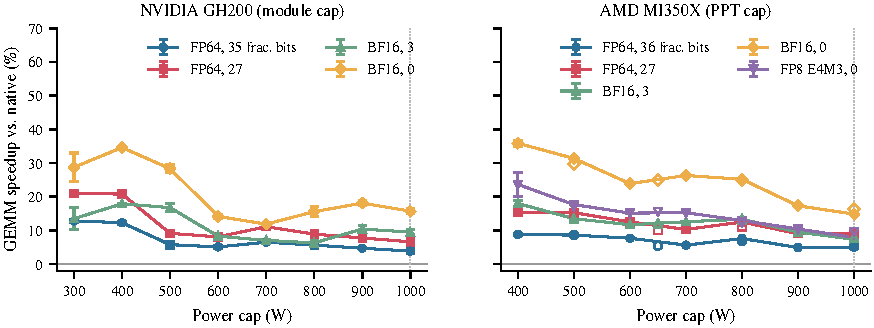
\includegraphics[width=\textwidth]{figs/mi350_gemm_caps.pdf}
\caption{GEMM speedup from mantissa zeroing under power caps. GH200 (module cap; FP64 $32768^2{\times}2048$, BF16 $k=6144$):
95\pct{} $t$ intervals over 6 node--pair samples (3 nodes $\times$ 2 ABBA pairs). MI350X (package cap; BF16 and FP8
$k=8192$): mean of node n02's two measurement windows, each averaging the 8 GPUs that run at once; bars span the two
windows; open markers: node n01. The dotted line marks each platform's default limit, which is also its highest.}\label{fig:gemm}
\end{figure*}

Zeroing speeds up GEMM at every cap on both platforms, though not monotonically as the cap tightens (Fig.~\ref{fig:gemm}).
On GH200, FP64 with 27 bits is 8.1--11.1\pct{} faster at 500--800\W{} ($\Delta W$ 79--162\W) and BF16 with 0 bits
11.9--28.3\pct. On MI350X the default limit already binds: at 1000\W{} FP64 with 36, 27 and 0 kept bits is 5.1, 9.2 and
16.9\pct{} faster, BF16 with 3 and 0 bits 7.7 and 15.6\pct, and FP8 with 0 bits 8.8\pct{} (means over the 4 measurement
windows of both nodes, 95\pct{} intervals $\pm$0.6--1.6 points); at 500\W{} the same are 8.6, 15.2, 60.0, 13.5, 30.6 and
17.4\pct{} ($\pm$0.1--1.5). The two nodes agree within 1.8 points, and temperature adjustment changes no value by more than
1.1 points. The equivalent saving per GPU is 42--72\W{} for FP64 with 36 bits at 600--900\W.

\subsection{HPL and HPL-MxP}\label{sec:hpl}

\begin{table}[t]
\caption{HPL scaled residuals (threshold 16; repeated runs reproduce exactly). Bits are significand bits including
the hidden bit (36 bits = 35 fraction bits), rounded to nearest even. GH200: 8 nodes at 1000\W, $N=286720$ is the tuned
configuration of the cap sweep; MI350X: one node of 8 GPUs at 1000\W. (F): fails the check; bold: the failures that
rule out 28 bits.}\label{tab:hpl}
\centering\footnotesize\setlength{\tabcolsep}{3pt}
\begin{tabular}{@{}lrrrrrr@{}}
\toprule
$N$ & Native & 36 bits & 32 bits & 30 bits & 28 bits & 24 bits \\
\midrule
\multicolumn{7}{@{}l}{\emph{GH200}} \\
131072 & $\ee{1.5}{-4}$ & 0.16 & --- & --- & 13.97 & 456 (F) \\
196608 & $\ee{1.3}{-4}$ & 0.072 & --- & --- & \textbf{18.09 (F)} & 462 (F) \\
262144 & $\ee{2.6}{-5}$ & 0.042 & --- & --- & 14.70 & 91 (F) \\
286720 & $\ee{7.6}{-5}$ & 0.038 & --- & --- & 15.40 & --- \\
\multicolumn{7}{@{}l}{\emph{MI350X}} \\
262144 & $\ee{5.4}{-5}$ & 0.46 & 11.1 & 84 (F) & \textbf{514 (F)} & --- \\
393216 & $\ee{4.6}{-5}$ & 0.15 & 12.0 & 20.2 (F) & \textbf{104 (F)} & --- \\
540672 & $\ee{7.8}{-6}$ & 0.27 & 3.5 & 17.3 (F) & \textbf{102 (F)} & --- \\
\bottomrule
\end{tabular}
\end{table}

The residual check determines the usable bit count, must be checked at several sizes, and depends on the platform
(Table~\ref{tab:hpl}). On GH200 28 bits sits within one bit of the threshold; on MI350X it fails at every size, by
6--32$\times$, and so does 30 bits. 36 bits passes on both with a margin of 35--100$\times$; the platforms differ in HPL
build and DGEMM blocking and accumulation order, so a bit count validated on one does not transfer.

\textbf{GH200, 8 nodes.} Tuned native HPL reaches 393.9\,TFLOP/s at 1000\W. With 36 bits it is 3.3--4.7\pct{} faster at
500--800\W{} over 6 pairs from two node sets measured on different days ($\Delta W=42$--74\W{} per node at 500--700\W),
and at the default cap mainly saves energy (7.5--8.6\pct{} per solve) with 0.6--3.9\pct{} more speed, depending on how far
the cap and temperature pull the native clock down. The node sets differ by up to 0.9 points, more than pairs within a
set, so node sets are the larger source of uncertainty (details in Supplement~S6). HPL-MxP with 3 kept bits is
1.7--5.8\pct{} faster at 500--800\W; refinement grows from 1 to 3 iterations, which eats most of the LU's 5--16\pct{}
speedup above 600\W; at 1000\W{} native HPL-MxP trips the chassis power brake at full fan speed, so we exclude that cap.

\begin{table*}[t]
\caption{MI350X: speedup (\%) over the unmodified program at the default limit and at 500\W. Pooled: mean $\pm$ 95\pct{} $t$
interval over the independent units of both nodes (window: one measurement window with the 8 GPUs averaged; run: one
node-wide run; round: one round of 8 GPUs). Per node: raw (same cooling environment) / adjusted to equal junction
temperature.}\label{tab:robust}
\centering\footnotesize\setlength{\tabcolsep}{4pt}
\begin{tabular}{@{}llcccccc@{}}
\toprule
& & \multicolumn{3}{c}{1000\W} & \multicolumn{3}{c}{500\W} \\
\cmidrule(lr){3-5}\cmidrule(l){6-8}
Result & Unit, $n$ & Pooled & n01 raw/adj. & n02 raw/adj. & Pooled & n01 raw/adj. & n02 raw/adj. \\
\midrule
GEMM FP64, 36 bits & window, 4 & $5.1\pm0.6$ & 5.2/5.4 & 5.0/5.5 & $8.6\pm0.1$ & 8.6/8.6 & 8.6/8.7 \\
GEMM BF16, 0 bits & window, 4 & $15.6\pm1.4$ & 16.4/16.6 & 14.8/15.2 & $30.6\pm1.5$ & 29.8/29.4 & 31.4/31.6 \\
GEMM FP8, 0 bits & window, 4 & $8.7\pm1.6$ & 9.6/9.5 & 7.9/7.9 & $17.4\pm0.6$ & 17.1/17.2 & 17.7/17.7 \\
HPL, 36 bits & run, 6 & $4.8\pm0.3$ & 4.6/4.5 & 5.1/4.8 & $7.0\pm0.6$ & 7.3/7.2 & 6.3/6.5 \\
HPL-MxP, 3 bits & run, 8 & $5.0\pm0.4$ & 4.9/4.8 & 5.1/5.1 & $19.3\pm1.3$ & 19.5/18.8 & 19.1/21.3 \\
GP likelihood, 28 bits & round, 4 & $7.4\pm0.6$ & 7.6/7.1 & 7.1/7.3 & $11.0\pm1.0$ & 10.8/12.5 & 11.2/12.9 \\
DF-MP2, 20 bits & round, 4 & $10.3\pm0.6$ & 10.2/13.3 & 10.4/14.2 & $18.6\pm0.3$ & 18.8/19.8 & 18.5/20.0 \\
DF-MP2, 32 bits & round, 4 & $5.7\pm0.4$ & 5.5/7.5 & 5.9/7.4 & $9.8\pm0.1$ & 9.7/10.5 & 9.8/11.0 \\
\bottomrule
\end{tabular}
\end{table*}

\begin{figure}[t]
\centering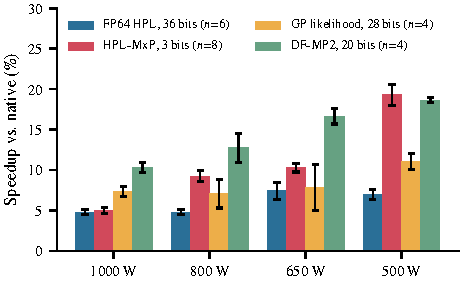
\includegraphics[width=\columnwidth]{figs/mi350_apps.pdf}
\caption{MI350X: speedup of the in-program truncated variant over the unmodified program under each package cap, both
nodes pooled. Bars: 95\pct{} $t$ intervals over independent units, node-wide runs (HPL, HPL-MxP) or rounds of 8 GPUs
(GP, DF-MP2), with $n$ in the legend; per-node and temperature-adjusted values in Table~\ref{tab:robust}.}\label{fig:mi350apps}
\end{figure}

\textbf{MI350X, one node of 8 GPUs.} Native HPL reaches 424.9 and 429.8\,TFLOP/s on the two nodes at 1000\W. With 36 bits
it is 4.6--5.1\pct{} faster at the default limit, 4.5--4.9\pct{} at 800\W, 6.2--8.0\pct{} at 650\W{} and 6.3--7.3\pct{} at
500\W{} (Table~\ref{tab:robust}), with 4.6--6.8\pct{} less energy per solve and $\Delta W$ of 39--50\W{} per GPU at
650--800\W{} (about 0.35--0.4\,kW per node). HPL-MxP, 7.61 and 7.65\,PFLOP/s natively, reaches 7.98 and
8.04\,PFLOP/s with 3 kept bits at the default limit (+4.9 and +5.1\pct) and gains 9.2--19.5\pct{} at 500--800\W, with
5.3--14.6\pct{} less energy per solve. Refinement grows from 2 to 4 steps (about 1.5\pct{} of the LU time). Keeping 0 bits
does not converge on MI350X, so 3 bits is the operating point on both platforms. The fan pitfall of
Section~\ref{sec:setup} biased one cell: on node n01 at 800\W{} all four 4-bit runs were about 12\,\textdegree C cooler,
and 4 bits appeared faster than 3 (+11.3 versus +9.3\pct); adjusted for temperature, 3 bits is +9.0\pct{} in that job,
+9.1\pct{} in a pairwise rerun and +9.1\pct{} on n02, and 4 bits +4.4--6.2\pct. Every other HPL and HPL-MxP cell moves by at most
0.7 points under the adjustment. For GP and DF-MP2 the adjusted gains are 0--4 points larger than the raw ones
(Table~\ref{tab:robust}): their variants run back to back in one process (native, 32/36 bits, 20/28 bits, then in reverse),
so the truncated variants occupy the middle, hottest part of each round, and the raw gains, which we report, are
conservative. All HPL-MxP results hold for the diagonally dominant test matrix only: the code's
generator always sets the diagonal to the row's absolute sum, and we have no implementation of a generator allowed for
official runs, so neither the 3-bit operating point nor its gain is a general property of HPL-MxP. They do not, however, depend on the
approximate factorization of the diagonal tiles: with exact factorization (\texttt{-{}-exact-diag}, node n02, one ABBA
pair), 3 bits passes the residual check (0.43) and is 4.4\pct{} faster at 1000\W{} and 9.4\pct{} at 650\W{}
(temperature-adjusted 4.4 and 9.3\pct), against 5.1 and 9.7\pct{} with the approximate factorization.

\subsection{Quantum ESPRESSO: Tolerance-Driven Bit Counts (GH200)}\label{sec:adaptive}

\begin{table}[t]
\caption{Quantum ESPRESSO with in-program truncation (round to nearest) of Davidson blocks: one uncounted warm-up run,
then mean $\pm$ 95\pct{} $t$ interval over 6 interleaved pairs; native rows give the mean of the 6 native runs. Energy
integrates 1-s averaged module power.}\label{tab:qe}
\centering\footnotesize\setlength{\tabcolsep}{2.5pt}
\begin{tabular}{@{}llrrcc@{}}
\toprule
System & Setting & Time & Energy & $\Delta E$ (Ry) & SCF \\
\midrule
\multirow{3}{*}{\shortstack[l]{Au\,112\\(450\W)}} & Native & 91.4\,s & 35.2\,kJ & --- & 28 \\
 & Adapt.\ $m{=}0$ & $-3.6\pm0.2\pct$ & $-3.4\pm0.1\pct$ & $<10^{-8}$ & 28 \\
 & Fixed 24 & $-2.0\pm0.2\pct$ & $-2.1\pm0.1\pct$ & $3{\times}10^{-8}$ & 28 \\
\midrule
\multirow{3}{*}{\shortstack[l]{Si\,1000\\(550\W)}} & Native & 205.7\,s & 108.4\,kJ & --- & 24 \\
 & Adapt.\ $m{=}0$ & $-2.1\pm0.1\pct$ & $-2.2\pm0.1\pct$ & $<10^{-8}$ & 24 \\
 & Fixed 28 & $-2.0\pm0.1\pct$ & $-2.1\pm0.2\pct$ & $<10^{-8}$ & 24 \\
\bottomrule
\end{tabular}
\end{table}

Plane-wave DFT tolerates 20--28 kept bits; Gaussian-basis DFT needs 32--36 (Supplement~S1). Tying the bit count to the
Davidson threshold, in-program, reproduces the native total energy in every printed digit ($10^{-8}$\Ry) on both systems
with the same SCF iteration count, while cutting time by 2.1--3.6\pct{} and energy by 2.2--3.4\pct{} against the unmodified
program (Table~\ref{tab:qe}); $k$ rises from 16 to 39--42 as the SCF converges. On the gold surface about half of the gain
comes from 7--9\pct{} fewer Davidson iterations, for reasons not yet identified; on Si\,1000 the work is unchanged, so its
2.1\pct{} is a power effect. The rule needs no safe bit count in advance and matches or beats the best fixed count.

\subsection{A Power-Hungry Application: DF-MP2}\label{sec:mp2}

\begin{table}[t]
\caption{DF-MP2 (taxol def2-TZVP): speed relative to native (mean $\pm$ 95\pct{} $t$ interval; GH200: 6 rounds from two
jobs on two nodes; MI350X: 4 rounds of 8 GPUs, two per node on two nodes), and the error $|\Delta E|$ of the MP2 correlation
energy (truncated variants round to nearest). MI350X GEMMul8 times exclude a one-time warm-up (Section~\ref{sec:crossover}).}\label{tab:mp2}
\centering\footnotesize\setlength{\tabcolsep}{2.0pt}
\begin{tabular}{@{}lrlll@{}}
\toprule
Cap & Native & 32 bits & 20 bits & Emulation \\
\midrule
\multicolumn{5}{@{}l}{\emph{GH200} (emulation: cuBLAS, 32 bits)} \\
1000\W & 39.5\,s & $+0.5\pm0.2\pct$ & $+0.8\pm0.1\pct$ & $-35\pct$ \\
700\W & 43.9\,s & $+4.9\pm0.4\pct$ & $+7.4\pm0.4\pct$ & $-28\pct$ \\
500\W & 51.5\,s & $+4.7\pm0.2\pct$ & $+7.7\pm0.5\pct$ & $-18\pct$ \\
\multicolumn{5}{@{}l}{\emph{MI350X} (emulation: GEMMul8, 12 moduli)} \\
1000\W & 21.7\,s & $+5.7\pm0.4\pct$ & $+10.3\pm0.6\pct$ & $+66.6\pm1.1\pct$ \\
800\W & 26.4\,s & $+6.7\pm1.4\pct$ & $+12.7\pm1.8\pct$ & $+60.7\pm0.9\pct$ \\
650\W & 34.1\,s & $+9.5\pm0.7\pct$ & $+16.6\pm0.9\pct$ & $+44.8\pm1.4\pct$ \\
500\W & 55.8\,s & $+9.8\pm0.1\pct$ & $+18.6\pm0.3\pct$ & $+32.6\pm3.1\pct$ \\
\midrule
$|\Delta E|$ & --- & $\le\ee{5}{-12}$ & $\le\ee{2.2}{-8}$ & G: $\ee{2.2}{-8}$; M: $\ee{7}{-12}$ \\
\bottomrule
\end{tabular}
\end{table}

The three-index tensor $B$ is zeroed in place once; the contraction $B_iB_j^{\mathsf T}$ (FP64 DGEMM with the auxiliary
basis as inner dimension, $k=5477$) dominates the run. Keeping 32 bits changes the MP2 correlation energy by at most
$\ee{5}{-12}$\Eh{} and 20 bits by at most $\ee{2.2}{-8}$\Eh{} (Table~\ref{tab:mp2}). On GH200 the truncated variants run at
native speed at 1000\W{} with 8--14\pct{} less energy and gain 5--8\pct{} under caps; on MI350X, held at the limit 95\pct{}
of the time at 1000\W, they are 5.7 and 10.3\pct{} faster there and 9.8 and 18.6\pct{} at 500\W{} (4 rounds on two nodes). Emulation behaves
differently on the two platforms (Section~\ref{sec:crossover}).

\subsection{A Wide-Range Workload: Gaussian-Process Likelihood}\label{sec:gp}

\begin{table}[t]
\caption{Gaussian-process likelihood ($n=80000$, six range parameters): largest log-likelihood deviation from native
and speed relative to native (mean $\pm$ 95\pct{} $t$ interval; GH200: 6 rounds; MI350X: 4 rounds of 8 GPUs on two nodes;
truncation rounds to nearest). The log-likelihoods are 1.2--1.7$\times10^5$. $^{a}$At $n=80000$ GEMMul8 returns success but an
invalid trailing update; at $n=64000$ it is 11--43\pct{} slower than native (Section~\ref{sec:crossover}).}\label{tab:gp}
\centering\footnotesize\setlength{\tabcolsep}{2.5pt}
\begin{tabular}{@{}lllll@{}}
\toprule
 & Trunc.\ 36 & Trunc.\ 28 & Emulation & FP32 \\
\midrule
\multicolumn{5}{@{}l}{\emph{GH200} (emulation: cuBLAS, 36 bits)} \\
$\max|\Delta\ell|$ & $\ee{2.4}{-5}$ & $\ee{7.2}{-4}$ & $\ee{2.2}{-3}$ & 87 \\
1000\W & $+3.0\pm0.3\pct$ & $+3.8\pm0.4\pct$ & $-41\pct$ & $-8.2\pct$ \\
700\W & $+5.0\pm0.1\pct$ & $+7.9\pm0.2\pct$ & $-31\pct$ & $+3.2\pct$ \\
500\W & $+4.8\pm0.1\pct$ & $+7.5\pm0.1\pct$ & $-21\pct$ & $+3.9\pct$ \\
\multicolumn{5}{@{}l}{\emph{MI350X} (emulation: GEMMul8)} \\
$\max|\Delta\ell|$ & $\ee{1.9}{-5}$ & $\ee{5.3}{-3}$ & wrong$^{a}$ & --- \\
1000\W & $+3.9\pm0.2\pct$ & $+7.4\pm0.6\pct$ & --- & --- \\
800\W & $+4.1\pm0.6\pct$ & $+7.1\pm1.8\pct$ & --- & --- \\
650\W & $+5.3\pm1.7\pct$ & $+7.8\pm2.8\pct$ & --- & --- \\
500\W & $+6.9\pm0.7\pct$ & $+11.0\pm1.0\pct$ & --- & --- \\
\bottomrule
\end{tabular}
\end{table}

The likelihood factors an $n{\times}n$ Matérn covariance by Cholesky; each panel $L_{21}$ keeps $k$ bits in one fused,
coalesced pass before its trailing update. The panel rows span 162 binades, and 88\pct{} of their nonzeros lie more than
$2^{-32}$ below their row maximum. With 28 bits the log-likelihood moves by a relative $\ee{3}{-8}$--$\ee{4.5}{-8}$, far below
what matters for estimation, and a one-parameter maximum-likelihood fit on GH200 returns the native estimate in every printed
digit (Supplement~S5). On GH200 the gain at 1000\W{} depends on how often native is capped (3.8\pct{} here, 0.1\pct{} with a
Morton ordering that is capped less); on MI350X the limit binds and 28 bits is $7.4\pm0.6\pct$ faster at 1000\W{} and $11.0\pm1.0\pct$ at 500\W{} (4 rounds on two
nodes). FP32 is unusable for estimation; truncating the FP64 tiles that remain in a tile mixed-precision Cholesky makes it a
further 1.9--7.0\pct{} faster, so truncation composes with format changes (Supplement~S5).

%==================================================================================================
\section{The Boundary with INT8 Emulation of FP64}\label{sec:format}

\begin{table}[t]
\caption{MI350X head-to-head: speedup over the best native run at the default limit / at 500\W, each method at the best
configuration it allows, with its error. Truncation: 36 bits (HPL), 35 (GEMM), 20 (DF-MP2), 28 (GP); GEMMul8: 10 moduli
(HPL), 12 (others). GEMM: $m=n=32768$.}\label{tab:h2h}
\centering\footnotesize\setlength{\tabcolsep}{2.2pt}
\begin{tabular}{@{}lll@{}}
\toprule
Workload & Truncation & GEMMul8 \\
\midrule
FP64 GEMM, $k=1024$ & +5.1/+9.2\pct{} ($\ee{8}{-12}$) & $-13$/$-45\pct$ ($\ee{4}{-13}$) \\
FP64 GEMM, $k=4096$ & +5.5/+9.0\pct{} ($\ee{8}{-12}$) & +84/+18\pct{} ($\ee{8}{-13}$) \\
HPL (residual) & +4.6/+7.3\pct{} (0.27) & +36/+11\pct{} (1.79) \\
DF-MP2 ($|\Delta E|$, E$_\mathrm{h}$) & +10/+19\pct{} ($\ee{2}{-8}$) & +67/+34\pct{} ($\ee{7}{-12}$) \\
GP, $n=64000$ ($|\Delta\ell|$) & +5.9/+11.8\pct{} ($\ee{2}{-3}$) & $-11$/$-43\pct$ ($\ee{3}{-7}$) \\
HPL-MxP (BF16) & +4.9/+19\pct{} (0.5) & no emulation \\
\bottomrule
\end{tabular}
\end{table}

Table~\ref{tab:h2h} sets the two methods side by side at the best configuration each allows. Emulation wins by a wide
margin where its fixed costs amortize at a generous cap (long inner dimensions: HPL, DF-MP2, GEMM with $k\ge2048$); a
tighter cap shrinks its lead or turns it into a loss; and it loses where the inner dimension is short (the
Gaussian-process likelihood and GEMM with $k=1024$). Truncation is smaller but positive everywhere, grows as the cap
tightens, needs no extra memory and applies to BF16 and FP8. The rest of this section explains the pattern.

\subsection{Crossover: Shape, Cap and Memory}\label{sec:crossover}

Emulation trades FP64 arithmetic for several times as many integer operations, so its benefit grows with the ratio of
INT8 to FP64 throughput, about 30 on GH200 and about twice that on MI350X. On GH200, cuBLAS emulation at the accuracy of
36-bit truncation ($\approx10^{-11}$) is 11--28\pct{} slower than truncation on a square GEMM with $k=2048$, and wins only
for long inner dimensions; across 480 measurements a three-parameter model in $1/m+1/n$ and $1/k$ describes GEMMul8 with
$R^2=0.98$--0.99 (Supplement~S4). On MI350X the crossover lies further toward emulation, and the cap moves it
(Fig.~\ref{fig:mi350xover}). Truncation to 35 bits ($\ee{7.8}{-12}$) is 5--6\pct{} faster than native at 1000\W{} and
8--9\pct{} at 500\W{} for every $k$. GEMMul8 with 12 moduli (more accurate, $\approx\ee{5}{-13}$) is 13\pct{} slower than
native at $k=1024$ but 36, 84 and 121\pct{} faster at $k=2048$, 4096 and 8192 at 1000\W; at 500\W{} these become $-45$,
$-18$, +18 and +48\pct. At $k=2048$ emulation wins at 1000 and 700\W{} and truncation at 500\W. Emulation draws the full
limit, so under a cap its extra integer work is paid for with clock, whereas truncation removes work from the power budget;
on GH200 the same holds for GEMMul8, while cuBLAS emulation, which draws only about 706\W{} at 1000\W, gains ground at lower
caps: the direction depends on the emulation's own power.

\begin{figure*}[t]
\centering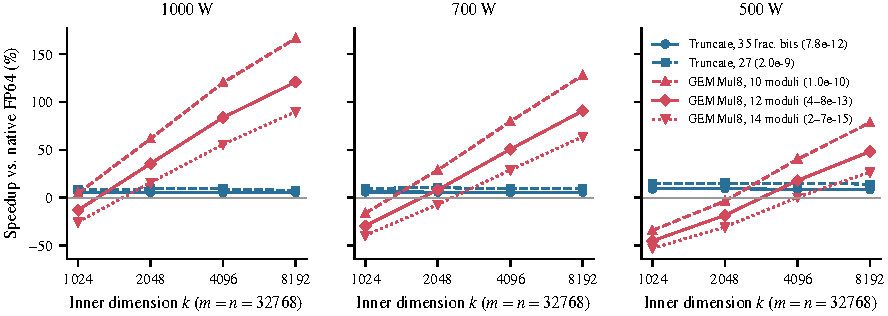
\includegraphics[width=\textwidth]{figs/mi350_crossover.pdf}
\caption{MI350X: speedup over native FP64 of truncation (round to nearest) and GEMMul8 for $m=n=32768$ as a function of
the inner dimension $k$, at three package caps (node n02, 8 GPUs $\times$ ABBA). A tighter cap lowers every emulation
curve and raises every truncation curve.}\label{fig:mi350xover}
\end{figure*}

\textbf{Applications.} In DF-MP2 on MI350X ($k=5477$) GEMMul8 with 12 moduli is 34--67\pct{} faster than native and beats
truncation at every cap, its lead over 20-bit truncation shrinking from 57 to 16 points between 1000 and 500\W; on GH200
cuBLAS emulation is 18--35\pct{} slower than native there (Table~\ref{tab:mp2}). In FP64 HPL on MI350X, GEMMul8 with 10
moduli on its own best configuration ($N=491520$, NB 4096, $4\times2$; residual 1.79 against 0.03 for 36 bits) reaches
576.8\,TFLOP/s at 1000\W, 36\pct{} above the best native configuration, but its lead over the best truncated run shrinks
from 30\pct{} at 1000\W{} to 4\pct{} at 500\W. \pending{12 moduli at $N=458752$ (job 64)}. In the Gaussian-process
likelihood, whose trailing updates have $k=1024$, GEMMul8 is slower than native at every cap ($n=64000$, where it is
correct: $-11$, $-22$, $-37$ and $-43\pct$ at 1000, 800, 650 and 500\W{} with 12 moduli, log-likelihood within
$\ee{3}{-7}$), while 28-bit truncation gains 5.9--11.8\pct.

\textbf{Costs that appear only in applications.} Emulation needs workspace: at the $N=540672$ of our best native HPL
configuration the matrix fills 292\,GB per GPU and GEMMul8's workspace no longer fits; on a $1\times8$ grid it requests
100--114\,GB even at $N=458752$; with 12 moduli even $N=491520$ fails; HPL must give up problem size before emulation can
start. Each new GEMM shape costs GEMMul8 a large one-time setup: DF-MP2's first pass over its 226 shapes takes 142\,s
instead of 13\,s (the times above exclude this warm-up). And in the Gaussian-process likelihood at $n=80000$, the hooked DGEMM of the first trailing update ($m=n=78976$, $k=1024$)
returned success but an invalid result in every one of 256 runs, without a diagnostic. A minimal reproduction on uniform
operands localizes it exactly: through the library's direct API and through the hook alike, $C=AB^{\mathsf T}$ with $k=1024$
is correct ($\ee{1.6}{-15}$) for $m=n=65535$ and wrong (relative error 31, all entries finite) from $m=n=65536$, i.e., once
$mn$ reaches $2^{32}$, consistent with a 32-bit size overflow in the GEMMul8 3.2.0 HIP build we used. It is an
implementation defect, independent of the data, not a property of emulation; every other emulated result in this paper
stays below this size. It illustrates the risk of replacing a BLAS call wholesale: a configuration validated at one size
can fail silently at another.

\subsection{Exponent Span: When Emulation Silently Fails}\label{sec:span}

\begin{table}[t]
\caption{GH200, real data (1000\W): flop-weighted fraction of nonzeros more than $2^{-32}$ below their row maximum, and the
total-energy error of each method. The ``Nearest'' rows keep 36 or 32 bits with round-to-nearest; cuBLAS emulation
with 36 and 32 bits uses five slices, with 40 bits six; auto: its automatic mode (at most 79 bits). The Au\,112
fraction comes from a two-iteration benchmark input, its errors from the fully converged input.}\label{tab:span}
\centering\footnotesize\setlength{\tabcolsep}{4pt}
\begin{tabular}{@{}llll@{}}
\toprule
& Valinomycin & QE Si\,1000 & QE Au\,112 \\
\midrule
Below $2^{-32}$ & 24--44\pct & 0.24--0.54\pct & 0.008--0.02\pct \\
Nearest, 36 bits & $\ee{9.6}{-7}$\Eh & 0\Ry & 0\Ry \\
Nearest, 32 bits & $\ee{1.2}{-5}$\Eh & 0\Ry & $\ee{4}{-8}$\Ry \\
cuBLAS emu., 36/32 & $\mathbf{\ee{5.25}{-2}}$\,\textbf{E}$_\mathbf{h}$ & $\ee{6}{-8}$\Ry & $\ee{5}{-8}$\Ry \\
cuBLAS emu., 40 & $\ee{8.4}{-8}$\Eh & --- & --- \\
cuBLAS emu., auto & $\ee{4}{-9}$\Eh & --- & --- \\
GEMMul8, 10 moduli & diverges & out of memory & $\ee{3.7}{-7}$\Ry \\
\bottomrule
\end{tabular}
\end{table}

Truncation keeps every element's exponent; Ozaki-type emulation slices each row relative to its maximum, so elements far
below the maximum lose bits. On data with a wide per-row span this can go wrong silently (Table~\ref{tab:span}): in
Gaussian-basis DFT on GH200, where 24--44\pct{} of the flop-weighted nonzeros lie more than $2^{-32}$ below their row
maximum, fixed 36-bit cuBLAS emulation lets the SCF converge normally to a total energy 52.5\,mE$_\mathrm{h}$ off, and
GEMMul8 diverges, whereas rounding to 36 bits errs by $\ee{9.6}{-7}$\Eh. With 40 bits or the automatic mode the emulation is
correct but 1.5--2.1$\times$ slower than truncation or native. Uniform synthetic spreads understate the problem: on both
platforms, spreading element exponents uniformly over up to 64 (MI350X) or 256 (GH200) binades barely affects GEMMul8
(MI350X, 12 moduli: median error $\ee{5.7}{-13}$--$\ee{8.0}{-13}$, p99 at most $\ee{4.4}{-11}$). A wide per-row span, which
an interposer can measure cheaply beforehand (Fig.~\ref{fig:map}), is therefore a necessary but not sufficient condition for
this kind of failure, the precision loss of a fixed-width emulation; narrow-span codes such as HPL, Quantum ESPRESSO and
DF-MP2 do not suffer it. It does not cover implementation defects such as the size overflow of Section~\ref{sec:crossover}, which occurs on
narrow-range uniform operands as well. Replacing every FP64 GEMM with FP32 or
3xTF32 fails for a different reason, accumulation over long inner products (Quantum ESPRESSO, Supplement~S3).

\begin{figure}[t]
\centering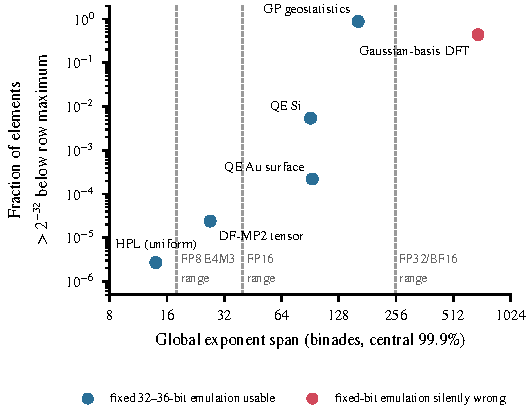
\includegraphics[width=\columnwidth]{figs/range_map.pdf}
\caption{GH200: global exponent span (central 99.9\pct) against the flop-weighted fraction of elements more than $2^{-32}$
below their row maximum, with the measured outcome of fixed 32--36-bit cuBLAS emulation (e.g., HPL: residual 0.197,
passes; Gaussian-basis DFT: 52.5\,mE$_\mathrm{h}$ error; Gaussian process: global span 162, estimate unchanged). All
points are measured; coordinates and their sources are listed in
\texttt{gh200/results/range\_map\_points.csv}.}\label{fig:map}
\end{figure}

\textbf{Truncation inside emulation.} Truncating the operands before GEMMul8 might lower the INT8 engines' toggling. On
MI350X it adds 1--4 points under a cap (12 moduli: 18.4 to 22.6\pct{} over native at 500\W{} with 19-bit operands) and
nothing at 1000\W, while the error becomes that of the truncation ($\ee{5.1}{-7}$); 8 moduli on full operands are faster and
more accurate. Within emulation, the number of moduli is the knob to turn.

%==================================================================================================
\section{Discussion}\label{sec:discussion}

\textbf{Where truncation pays.} Three conditions decide the gain: the GPU must be power-bound, the truncated operands
must flow directly and in volume into multipliers or data paths, and the algorithm must tolerate the error, ideally by
correcting it. The model makes the first quantitative; the second explains why GEMM-dominated solvers gain 4--20\pct{} while
codes whose intermediates regrow full mantissas (N-body, MFEM, SW4, LAMMPS) gain little; the third separates HPC solvers
from AI weights. On GH200 the gain at the default cap is mainly energy; on MI350X, whose default limit binds for FP64, BF16
and FP8 matrix work, truncation turns into 4.6--10\pct{} more speed at stock settings. As throughput grows faster than
power envelopes, running at the limit becomes the default operating point, and the energy spent toggling unneeded bits
becomes a first-order performance parameter.

\textbf{Truncation and emulation.} Emulation is the stronger lever where it can amortize its fixed costs: long inner
dimensions, generous caps, narrow exponent spans, ample memory and few distinct shapes. Truncation is the better choice
elsewhere, and the only one outside matrix multiplication and for BF16 and FP8, for which no emulation exists. A runtime
that knows each call's shape, the cap and a cheap span estimate could choose per call.

\textbf{AI workloads.} Truncation does not carry over to model weights, which no residual corrects. Truncating the frozen
FP8 base weights of Llama\,2 70B LoRA fine-tuning to 2 of 3 mantissa bits made each step 0.9--1.2\pct{} faster but needed
22--39\pct{} more samples to reach the target loss (two seeds); in inference BF16 with 3 kept bits matches FP8's accuracy on
six language models while FP8 GEMMs are 1.7--1.9$\times$ as fast, and zeroing on top of FP8 saves only 1.5--5.5\pct{} of
power at an accuracy cost (GH200; Supplement~S7). Whether reduced precision improves time to target quality under power
limits needs its own study.

\textbf{Benchmark rules.} TOP500 rules require full FP64 arithmetic~\cite{TOP500Linpack}, and HPL-MxP rules require at
least 16-bit floating point and allow diagonally dominant matrices for testing only~\cite{HPLMxPRules}; all HPL and HPL-MxP
numbers here are research results, not official scores. Scientific software has no such restriction; the criterion is
whether physical results stay within the required accuracy.

\textbf{Limitations.} (i)~Two platforms, one generation each, and single-node (8-GPU) runs on MI350X; other parts manage
power and cool differently. (ii)~Safe bit counts depend on platform and problem size and must be validated (HPL 28 bits:
passes on GH200 at three of four sizes, fails on MI350X at all). (iii)~HPL-MxP results hold for a diagonally dominant test
matrix only. (iv)~Each scientific code was tested on one or two inputs; on MI350X DF-MP2 uses our own contraction of
PySCF's tensor. (v)~Units of independence are runs, windows or rounds within one or two nodes; GH200 intervals treat pairs
within a node set as independent, and node sets differed more than pairs within a set. (vi)~Temperature confounds
power-capped measurements; ABBA cancels linear drift but not fan feedback, so we report temperature-adjusted values beside
raw ones. (vii)~Default caps are also the highest, not uncapped states, and the limiters' time scales are unknown.
(viii)~Power and energy come from the devices' own sensors and accumulators, not an external meter; GH200 module power
includes the Grace CPU. (ix)~The MI350X clock reduction attributed to clock stretching is an inference. (x)~About half of
the Quantum ESPRESSO gain on the gold surface comes from fewer Davidson iterations, for unidentified reasons. (xi)~The
GEMMul8 failures (memory, silent invalid result) are observations about one library build.

\section{Conclusion}\label{sec:conclusion}

On GPUs of two vendors, truncating unused mantissa bits in software buys performance for HPC applications under power
limits while their results stay within each code's own criterion. Bits that stop toggling account for most of the saved
energy, and a simple model built on this predicts a truncated kernel's performance--cap curve from the native curve, the
idle power and one or two measurements. MI350X is power-bound at its stock limit, so truncation speeds up HPL, HPL-MxP on
a diagonally dominant test matrix, a Gaussian-process likelihood and DF-MP2 by 4.6--10\pct{} at default settings and
7--19\pct{} at 500\W. It is one of two ways to spend less energy per useful FP64 operation, and not the faster one
everywhere: INT8 emulation leads by up to 67\pct{} where long inner dimensions amortize its fixed costs at a generous cap,
while short inner dimensions, tight caps, full memory, many distinct shapes and wide per-row exponent spans favor
truncation, which also keeps the format, needs no extra memory and applies to BF16 and FP8. Safe bit counts must be
validated on the target platform, and power-capped measurements must control temperature. All HPL and HPL-MxP numbers are
research results, not official scores.

% Data and code availability: to be added before submission (anonymized for double-blind review).

\bibliographystyle{IEEEtran}
\bibliography{refs}

\end{document}
